\appendix

\section{Experimental details and extraction ablations}

\paragraph{A magnitude-matched null, and why the obvious one fails.}
The natural correction projects the latent back toward the level set,
$z \leftarrow z - \alpha (C(z) - C_0)\,\nabla C / \lVert \nabla C \rVert^2$. This is a Newton step, so
its size grows with how badly the constraint is violated --- and a random constraint is violated far
more than a conserved one. Matching random draws in \emph{coefficient} norm, as one might expect to
control for scale, controls nothing: the step is invariant under $C \to \lambda C$. Measured, random
draws take steps $29\times$ larger than the recovered constraint, so the comparison conflates
direction with magnitude.

We therefore fix the step size and vary only direction,
$z \leftarrow z - \varepsilon\,\mathrm{sign}(C - C_0)\,\nabla C / \lVert \nabla C \rVert$, over a
frozen $\varepsilon$ grid. Arms then differ in where they push, never in how hard.

\paragraph{Three kinds of latent trajectories.} We use three latent trajectories and keep them
separate throughout.

An \emph{observation-conditioned} trajectory is the sequence of deterministic recurrent states
produced when the model receives the next real frame at every step. This is what the encoder returns
on the analysis set.

The \emph{one-step transition} $T$ is the model's autonomous recurrent update with zero action and
no new observation.

An \emph{imagination rollout} starts from one encoded state and repeatedly applies $T$ without
supplying any later frames.

We estimate the latent flow by applying $T$ once at each state of an observation-conditioned
trajectory, so the transition is autonomous even though the states come from real video.
Section~\ref{sec:dissociation} measures conservation along observation-conditioned trajectories.
Section~\ref{sec:causality} tests what happens to the same scalar under autonomous imagination.

\paragraph{Code and data.} The extraction code, the run logs behind every figure and table, and
the source of this paper are at \url{https://github.com/Zarand3r/world-model-invariants}. The figures
regenerate from the committed logs without a GPU.

\paragraph{Preliminary experiments.} We developed the extraction procedure in preliminary
experiments on smaller recurrent models. Those experiments motivated the untrained, dissipative, and
intervention controls used here, and we do not use them as evidence for the DreamerV3 results.

\label{sec:details}

\paragraph{Training.} We set free bits to 0 rather than DreamerV3's reference default of 1.0. The
measured KL divergence settles near 1.8 nats, well above collapse, so the floor is inactive here. All
three trained models pass the acceptance checks; none were discarded.

\paragraph{Data split.} Training uses trajectories 0--203 of the 256-trajectory dataset. The
remaining 52 form the analysis set. We fit $C$ on those 52 trajectories and evaluate the
Section~\ref{sec:causality} correction on the same 52, so the absolute effect is in-sample with
respect to invariant fitting. The recovered and random-constraint arms use the same trajectories.

\paragraph{Scoring the correction over a grid.} We score the slope of rollout error over the fixed
$\alpha$ grid rather than the minimum on that grid. Taking the minimum selects the most favourable of
five points after seeing the curve. In one diagnostic run that rule would have reported a 5.9\%
improvement for an arm whose error rose monotonically to twice baseline.

\paragraph{Flow alignment contributes reproducibility.} Holding the candidate family, data,
dimension, degree, and $\alpha$ grid fixed, we select $C$ either by the invariance criterion alone or
by the joint criterion. Conservation alone recovers energy at $0.950$ against $0.973$ for the joint
rule, and gives a slightly better mean intervention slope ($-0.087$ against $-0.077$, winning on two
of three models). The difference is in spread: recovery varies by $0.035$ across seeds under
conservation alone and by $0.008$ under the joint rule.

\paragraph{The pairing residual does not track recovery.} As the extraction dimension rises from 6 to
12, energy recovery improves from $0.721$ to $0.967$ while the pairing residual worsens from $0.738$
to $0.876$. Recovery already reaches $0.967$ at dimension 8, where the residual is lower at $0.813$.
The added dimensions do not carry energy while resisting the Hamiltonian fit: directions 7--12
account for 44.9\% of the residual and 43.5\% of the flow. Figure~\ref{fig:ldsweep} gives the sweep.

\section{Causal-intervention protocols and per-model numbers}
\label{sec:causal-detail}

If the recovered scalar is only a descriptive correlate, enforcing it has no reason to help and
setting it has no reason to steer. Three interventions test the alternative, each with matched
controls.

\paragraph{A magnitude-matched null.}
Arms differ only in \emph{where} they push, never in how hard: we fix the step size and vary
direction, $z \leftarrow z - \varepsilon\,\mathrm{sign}(C - C_0)\,\nabla C / \lVert \nabla C \rVert$,
over a frozen $\varepsilon$ grid. The obvious alternative --- a level-set projection with random
draws matched in \emph{coefficient} norm --- controls nothing, because the step is invariant under
$C \to \lambda C$; measured, random draws then take steps $29\times$ larger than the recovered
constraint. Appendix~\ref{sec:details} gives the derivation.

\paragraph{Correcting the invariant repairs the imagined physics.}
We evaluate on decoded physical energy rather than pixels: a non-learned geometric readout recovers
$\theta$ by image moments and $\dot\theta$ by backward differences, matching the simulator's
semi-implicit convention, with median decoded-energy error $1.6\%$ of the across-trajectory spread.
The statistic is secular drift of decoded energy over a rollout.

At $H = 100$ the recovered direction reduces drift by 32--51\% across three models. On 512
trajectories from a disjoint generator seed, with $C$ and the entire coordinate frame frozen, the
effect does not shrink: $-54.6\%$, $-58.8\%$, $-75.9\%$ at $H = 190$. Across both horizons
\textbf{0 of 60} magnitude-matched random directions and \textbf{0 of 15} equal-norm tangent
directions beat the recovered one on any model.

\paragraph{Setting the invariant steers the imagined physics.}
Repair shows drift is costly, not that $C$ is a control variable. We move a recipient state minimally
along the local $C$-normal until $C(z) = C(z_{\mathrm{donor}})$ for an independent donor trajectory,
then let the rollout run free; the target is read from the model's own latent, never from true
energy. The imagined world's \emph{true decoded} energy moves toward the donor's \emph{true} energy,
rank correlation $0.802$--$0.914$ across three models, with \textbf{0 of 75} random and tangent
controls beating it and a preregistered offset sweep monotone in both directions on every model.

\paragraph{The subspace is used by the model's own dynamics, not only reachable from encoder states.}
A subspace edit can produce the expected output change through a pathway the model does not normally
use \citep{makelov2024illusion}, so we repeat the donor interchange \emph{50 steps into an autonomous
rollout} --- on a state the model reached by itself. The effect barely degrades: rank correlation
$0.762$--$0.849$ at depth 50 against $0.803$--$0.924$ at depth 0, with 0 of 13 controls beating it at
either depth, and equal-norm tangent edits near zero throughout. A dormant pathway would lose its
effect precisely where this test applies it.

\paragraph{The same pipeline refuses when there is nothing to find.}
On matched dissipative models, where no nontrivial first integral exists, the extraction returns a
direction that is not distinguished from a random one: 24 of 60 random draws beat it, and it harms
rollouts on 2 of 3 models. Its operator statistic sits at $3.4$--$3.7\times10^{-1}$, in the same range
as an untrained network and $39\times$ worse than any conservative model, with no overlap between the
two groups.


\paragraph{Downstream tests in full.}
\paragraph{No downstream benefit, and we measured why.}
Both practical uses we tested fail, for one reason. Planning with CEM over the learned model on an
energy-targeting task, scoring return from the simulator's true state, the model plans well ---
beating a random-action policy by $+1.65$, 95\% CI $[+0.50, +2.79]$. But no correction arm, including
one supplied with the action's power as a source term, differs from no correction over three models
and 20 episodes each: the largest effect is $0.0014$ against an across-episode return standard
deviation of $0.575$, \textbf{0.24\% of one episode's spread}, and all four registered predictions
failed. The cause is structural. The correction acts on \emph{accumulated} drift, and at the
planner's horizon it shifts imagined energy by $0.3\%$ of the spread across candidate action
sequences --- the quantity the planner ranks plans by --- so it cannot change which plan is chosen.
Our repair is measured over 100 autonomous steps; a controller that re-plans every step never
imagines long enough to accumulate what the method removes. Nor can one simply look further ahead:
tripling the horizon leaves every arm indistinguishable (largest effect $0.007$ against a return
standard deviation of $0.862$) while planning quality itself degrades, $-0.34$ to $-0.56$ in mean
return. The regime where the correction would have something to correct is the regime where the
planner is already worse off.

The same effect-size limit defeats the other use. Accumulated drift at rollout step 25 predicts
decoded energy error at step 100 at Spearman $-0.02$, $+0.09$ and $-0.24$, against $+0.27$, $+0.29$
and $+0.31$ for plain latent displacement, with a random-constraint control beating it on two of
three; the registered prediction went the other way on every model. A conserved quantity being
causally deployed in imagination does not imply its drift is a useful online signal. The effect on
pixel error alone is also small ($1.7\%$ at $H{=}50$); the large effects here are on decoded physical
energy, a metric we introduce because it measures the property in question.

\paragraph{The method finds only what the data gave the model a reason to represent.}
The pendulum's rod length is fixed, so the rendered bob's distance from the pivot is constant to
$0.67\%$ --- an exact constraint. Searching for a residual $G(z)=0$ rather than a conserved scalar
fails: the recovered direction correlates with the true residual at $0.004$--$0.032$. Two measured
causes. Minimising $\mathbb{E}[G^2]$ is the wrong objective, ranking the true constraint $1525$th of
$1819$ directions; and the constraint is barely encoded at all, predicted from the latent at held-out
$|\rho| = 0.19$ with a residual four times its own variation. A quantity that never varies carries no
information, so nothing in a reconstruction objective pushes it into the latent --- it can live in
the decoder's weights. This bounds the approach to quantities that \emph{vary}, and it is why we
report no released-checkpoint experiment: limb lengths do not vary either.

Finally, the two-invariant case limits the extraction rather than the model. On a system conserving
both energy and angular momentum the conserved subspace reliably contains both (angular-momentum
correlation $0.94$--$0.98$ in every measurement), while the joint fit isolates either in only 1 of 7
measurements. The flow-alignment criterion selects a single direction inside that subspace, and has
no unique answer when two independent invariants exist.


\paragraph{Conservation at matched decodability, in full.}
\paragraph{Whether conservation \emph{alone} predicts the intervention is not established.}
The control that would show this directly asks whether, among candidates matched in energy
correlation, better conservation alone produces a larger repair. The 2-DoF system admits such a band:
on two of three seeds, 397 and 398 of 400 candidates lie within $0.10$ of the recovered scalar's
$|\rho|_E$, spanning five orders of magnitude of conservation quality at $|\rho|_E \le 0.11$. Across
20 candidates stratified by conservation, the rank correlation with repair is $+0.19$, $+0.57$ and
$+0.19$ on the three seeds, with the 95\% confidence interval excluding zero on \textbf{one of
three}. We report this as a negative result: the relationship is visible but not established at
$n = 3$.

Two further facts belong with it. The point estimate moves with the size of the candidate pool
($+0.29 \to +0.19$ on one seed between pools of 150 and 400), so the statistic is not stable to a
design choice that should be immaterial --- though the one-of-three verdict is identical under both
pools. And on the third seed the band cannot be built at all: its reference $|\rho|_E$ is $0.111$ and
only 19 of 400 candidates fall within $0.10$ of it, with an increase from 150 to 400 candidates
adding none.

That last failure is the informative part. On a system whose transition conserves energy, the
well-conserved latent directions \emph{are} the energy-like ones. This is why E10's original
high-decodability form could not be constructed on the pendulum at any pool size, why the matched
band here exists only at low decodability, and why on one seed it does not exist at all. The two
properties may not be separable by this design on any system where the model has learned the physics.
That is a statement about the difficulty of \emph{this control}, not about the dissociation itself,
for which the supervised probe above and Section~\ref{sec:mechanism} give direct evidence. What does
hold across all three seeds is that the recovered scalar repairs: $-16.7\%$, $-7.3\%$ and $-6.8\%$.


\paragraph{Under actuation the same split appears against a different law.}
The four axes above vary how well a \emph{conserved} quantity survives; a fifth varies the law
itself. Three further models are trained on the same pendulum under piecewise-constant random torque,
where energy instead obeys $\mathrm{d}E/\mathrm{d}t = \tau\dot\theta$. They demonstrably use their
actions: a 20-step open-loop rollout under the true action sequence beats one under the same actions
shuffled across trajectories, $0.740$--$0.761$ on 3 of 3 seeds. The \emph{unchanged} extraction
recovers an energy-like scalar on every model ($|\rho|_E = 0.72$, $0.88$, $0.86$), yet its motion
under the model's own transition does not follow the balance relation: with the torque known and
$\dot\theta$ from the same decoded readout, the rank correlation with the predicted source term is
$0.041$, $0.076$ and $0.065$, the power term accounts for \textbf{0.31\%} of the variance in
$\Delta C$, and the observed change is $4.5$--$5.4\times$ larger than predicted. A shuffled-power
control is beaten 3 of 3, so the pairing carries something --- almost nothing. The model represents
the quantity and does not implement the relation it obeys, which is also why a correction built on
that scalar confers no control benefit (Section~\ref{sec:limits}): there is no balance structure for
it to enforce.


\paragraph{Where the phenomenon stops.}
Both boundaries above are the same statement seen twice. The invariant is bounded to the
\emph{training distribution}: outside the training energy band a freely fitted probe still recovers
energy at $0.999$ while the transition conserves it $55$--$267\times$ worse, reaching values
indistinguishable from a random constraint. And it is bounded to the \emph{architecture}: on a
deterministic convolutional GRU with no stochastic latent, no KL term and no unimix, identification
transfers on 2 of 3 seeds under both training budgets while conservation transfers on none
($\rho_{\mathrm{obs}}$ $4.83$--$5.55$ against the RSSM's ${\sim}7\times10^{-3}$, a $767\times$ gap;
seven times more open-loop training moved the median from $5.33$ to $5.26$). We are explicit that
this comparison does not isolate architecture --- an open-loop reconstruction term and a
prior--posterior KL are different losses, not the same loss at different strengths --- so the
supportable scope of every claim here is RSSM-like models, in distribution.

\section{Latent sensitivity analyses}
\label{sec:sensitivity}

For each direction $u$ of the extracted subspace we measure its variance and the damage a
displacement along it does to an imagination rollout,
\begin{equation}
V(u) = \operatorname{Var}(u^\top z), \qquad
D_H(u) = \mathbb{E}\bigl[L_H(z+\epsilon u) - L_H(z)\bigr],
\label{eq:leverage}
\end{equation}
with $L_H$ the $H$-step imagination error against the analysis set.

\paragraph{Calibrating the displacement.} At $\epsilon = 0.05|z|$ the damage is about $-0.5\%$ of
baseline with the sign varying across directions. Imagination is deterministic, so repeated
unperturbed rollouts are identical and these values are not sampling noise. Damage for the leading
direction runs $-0.5\%$, $+3.1\%$, $+18.1\%$, $+46.4\%$, and $+128.8\%$ at $\epsilon/|z|$ of $0.05$,
$0.10$, $0.25$, $0.50$, and $1.00$. We use $\epsilon = 0.25|z|$, the smallest displacement whose
damage exceeds 10\% of baseline while the response still grows smoothly.

A displacement does not decay under imagination. After 40 steps it retains $6.3\times$ its initial
size at $\epsilon = 0.05|z|$, $2.8\times$ at $0.25|z|$, and $1.9\times$ at $0.5|z|$, as medians over
the three models.

\paragraph{Variance and sensitivity at different horizons.} At a 40-step horizon the two rankings
anticorrelate on all three models ($-0.364$, $-0.259$, $-0.406$), with damage spanning
$13.5\times$ to $118.8\times$ between the most and least consequential direction
(Figure~\ref{fig:leverage}a). The ranking replicates: split-half rank correlation of $D_H$ has median
$0.95$ across the settings we tried, with a minimum of $0.52$ at the smallest displacement and
longest horizon. The disagreement with variance does not extend to long horizons. Pooling three
models and three displacements, median $\rho(V, D_H)$ is $-0.252$ at horizon 20, negative in 9 of 9
settings; $-0.196$ at horizon 50, negative in 5 of 9; and $-0.028$ at horizon 100, negative in 5 of
9, with one setting reaching $+0.727$. Once a rollout has diverged, high-amplitude directions
dominate the error and the rankings realign.

The correction pushes along higher-damage directions at $+0.385$, $+0.692$, and $+0.287$
(Figure~\ref{fig:leverage}b), without having been given that ranking. The correlations stay well
below $1$, so the correction is only partly concentrated there. All of this is measured on the
conservative models.

\begin{figure}[h]
\centering
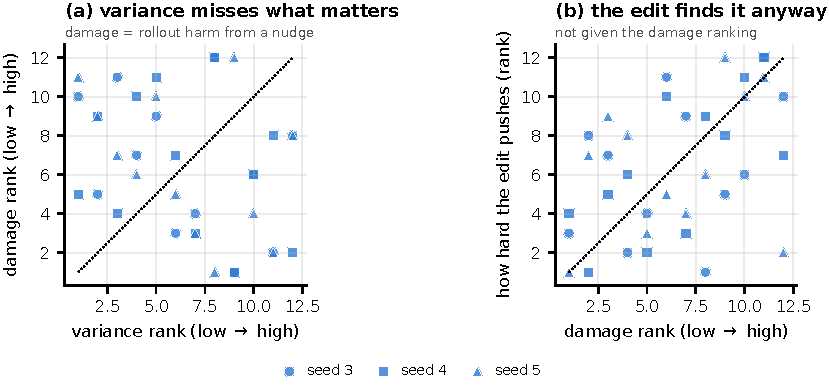
\includegraphics[width=\textwidth]{figures/fig3_leverage.pdf}
\caption{Each point is one of the 12 extracted directions, ranked within its own model; the dotted
line marks equal ranks. \textbf{(a)} Variance rank against damage rank at a 40-step horizon.
\textbf{(b)} Damage rank against the magnitude of the invariant correction along that direction.}
\label{fig:leverage}
\end{figure}

\paragraph{Basis-independent properties reproduce better than coordinate selectors.} The three models
agree closely on quantities that need no choice of basis: energy recovery varies by $0.008$,
intervention slopes by $0.016$, and the top-3 eigenvalue mass of
$M_C = \mathbb{E}[gg^\top/\|g\|^2]$ with $g = \nabla C$ by $0.046$ ($0.448$, $0.441$, $0.487$).
Selectors on individual coordinates are less stable: ranking coordinates by $\nabla C$ and keeping
the top three gives intervention slopes of $-0.075$, $+0.016$, and $-0.089$, beating a variance
ranking on two models and changing sign across seeds. An orthogonal projector onto the top eigenspace
of $M_C$ beats the variance selector on all three models, though on one it sits at the 41st
percentile of 100 random rank-3 subspaces. Since the correction is rank one at each state, the
spectrum of $M_C$ measures how much $\nabla C$ rotates as the state changes, and the amount is
similar across models. This is consistent with the models encoding the same scalar in different
latent coordinate systems, although we do not directly align their representations.

\section{Additional sweeps}
\label{sec:sweeps}

\paragraph{Energy outside the highest-variance directions.} On two of three models, principal
directions 7--12 carry about twice the energy information of the top six ($2.23\times$ and
$2.13\times$); on the third the ratio reverses to $0.91$. We report the models separately because a
median would hide the sign change. Figure~\ref{fig:lowvar} shows the decomposition.

\paragraph{Accumulated invariant error.} Accumulated invariant error predicts which rollouts degrade
most: an integral predictor reaches $R^2 = 0.187$ against $0.021$ for a fitted power law in time at
the horizon where both perform best, and shuffling destroys the relation. The current experiments do
not distinguish weighted from unweighted accumulation. In a nested comparison with 400 bootstrap
resamples, the weighted term adds explanatory power beyond the unweighted term in 1 of 9
seed--horizon combinations, and the unweighted beyond the weighted in 0 of 9, at $n = 512$.

\begin{figure}[h]
\centering
\begin{minipage}[t]{0.36\textwidth}
\centering
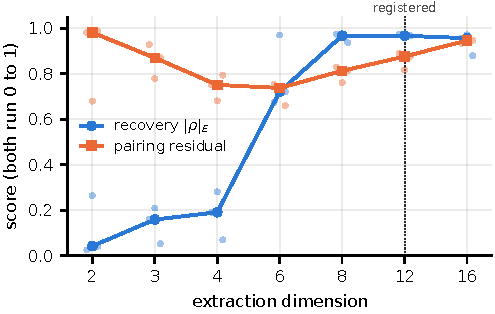
\includegraphics[width=\textwidth]{figures/fig4_ld_sweep.pdf}
\caption{Energy recovery and pairing residual against extraction dimension. Lines are medians over
the three models; points are individual models. Both quantities are dimensionless.}
\label{fig:ldsweep}
\end{minipage}\hfill
\begin{minipage}[t]{0.58\textwidth}
\centering
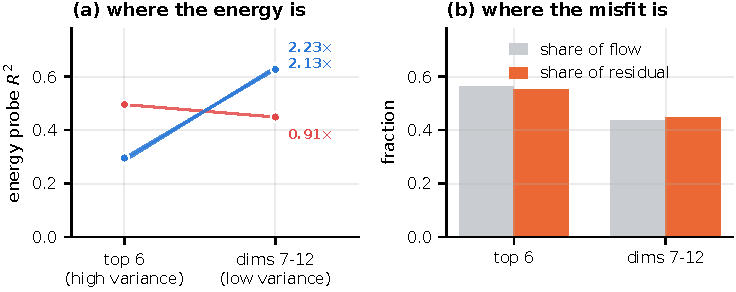
\includegraphics[width=\textwidth]{figures/fig5_low_variance.pdf}
\caption{\textbf{(a)} Energy-probe $R^2$ for the top six principal directions against directions
7--12, per model. \textbf{(b)} Fraction of latent flow and pairing residual carried by each group,
medians over three models.}
\label{fig:lowvar}
\end{minipage}
\end{figure}
